\chapter{Project Management}
\label{Project_Management}

\section{Winter Quarter Review}
Throughout the winter, we and our global team tried to explore our huge design space and identify which were the directions we should pursue and which we should eliminate. To do so we always tried to coordinate the work done at Stanford with the work done in Brazil. 

At the beginning of the quarter we wanted their project to explore one aspect of the flight experience while we were exploring something else. The idea was then to see which approaches were feasible and which were not. For instance changing the changing the cabin layout turns out to be impossible under the constraint of keeping the number of passengers onboard the same. But at some point, USP and us needed to converge that is what we did after coming back to some of our users’ interviews and need findings. 

We decided to create a new flight experience for disabled people that would start from the jet way where wheelchair passengers leave their wheelchair. At this point Stanford team decided to provide them with a protection system for their wheelchair as well as a wheelchair tracking device to reassure them and give them piece of mind. 

From the jetway, once the disabled person is in the wheelchair then he needs to transfer to his seat and to do so without the help of any flight attendant USP decided to focus on the transfer mechanism that would give our passengers more independence. 

Integrating both our prototype with USP’s, we were able to build our vision for next quarter. When a wheelchair user is without his wheelchair he worries about two things: what happens to his wheelchair, his legs, and how he can actually move without it. By merging our ideas with our global partners’ we should be able next quarter to build a prototype that should this issue.


\section{Deliverables}
%The official deliverables for the winter quarter focus on three main prototypes: dark horse, funky, and functional.  In addition to these three prototypes, our team has set more deliverables within each one.  Each prototype will have a dedicated brainstorming session after a project briefing, and two iterations of each prototype must be performed. The dark horse prototype is where we plan to address the futuristic cabin approach and bring that idea to life.  We want to have the basis of our final solution started by the end of dark horse and continually increasing to the end of winter quarter.  Our main personal deliverable will be to have a final solution design space and all the integral components decided before the end of winter so spring will be iteration after iteration until perfection. 

\section{Milestones}
%The milestones for the winter quarter are the darkhorse, funky, and functional prototypes.  Each of these will represent a challenge to our design thinking and our solution space.  In addition, we have the milestone of integrating two new team members into the ME310 experience and making a smooth transition.  Another milestone will be the creation of our final design solution space.  We will also be traveling to Brazil at the end of the winter quarter to do a prototype meeting. 

\section{Distributed team management}
The entire team will be working on each of these projects and doing the documentation that accompanies each one.  Each team segment will be responsible for the documentation concerning their prototypes and clearly articulating the lessons learned and the takeaways. We plan to continue write the documentation in paragraph and bullet form from the beginning next quarter instead of bullets to make an easier transition.  The bullet format will still be used to distribute ideas to our global team and the teaching team. Throughout this quarter, we have made an active effort to write up each section as the prototyping cycle ends. This way, all of the information is still fresh in our minds and we do not have to scramble at the end to finish it all on time. We will continue on this path as it has proven to be successful thus far. 



\section{Project Budget}
Figure \ref{fig:budget} shows our projected budget for this spring.

\begin{figure}[h]
\centering
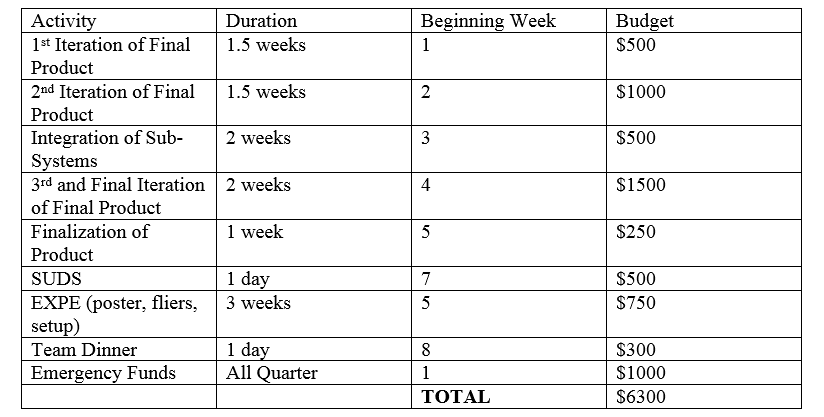
\includegraphics[width=7cm]{images/budget.png}
\caption{Spring budget}
\label{fig:budget}
\end{figure}


\section{Reflection and Goals}

\subsection{Laura Hoinville}
As a new member of the team it was a little hard for me to jump right into dark horse as a first prototype to build, but once I understood what were the expectations both from the class and from our users I found at that this project is a great opportunity to merge my engineering skills (I’m from an aerospace engineering background) with empathy and understanding of the needs and issues of people you are designing for. 

I know a lot of aircraft design because this is the field where I’d like to start my career, but anytime I was taught about it, it was mainly in terms of aircraft performance and never in terms of people’s need. I think this project is allows to see aircraft design from the user’s point of view instead of the aircraft manufacturer’s point of view and for me this is extremely valuable. 

Since I come from France it is actually the first time that I have the opportunity to work with both American and Brazilian people and this cultural diversity is also a great source of enrichment. I’m looking forward to go to Brazil to meet our global partners in person. 

But beyond this, this project now means a lot to me. I got the opportunity to talk to disabled people and understood how painful it is for them to travel. They care a lot about our project because they see it as way to improve their experience and I don’t want to disappoint them. They deserve the right to enjoy their flights the way we do and for this reason I’m very excited about Spring Quarter and I can’t wait to build our final prototype and test it.

\subsection{Maria Barrera}

This quarter was challenging and rewarding in many ways. As one of the members of the original team, it was my duty to introduce our new team members not only to our users and the project but also the class and the requirements themselves. I must admit that it was a very challenging beginning, especially since the confusion that came with being new to the class was magnified by our inability to choose a direction early on. 

While having 2 members at Stanford was hard, having 5 team members brings many different challenges along with is as well. Especially when these team members are thrown in at one of the most challenging parts of the quarter- dark horse. It was very hard to get people to take ownership and initiative when it came to projects or running meetings, particularly when none of us knew what our final goal was. We didn't know each other, we hadn't worked together before and many of us didn't know what to expect. We had to actively work to create a team dynamic we are now happy with yet this process has been just as tiring and effort consuming as the project itself. 

 I must admit I am now much more comfortable with ambiguity that I was when I first decided to take this class. I've learned to trust the journey, really listen to the user and not get attached to any one idea. I've learned to work with many different kinds of people and learned to lead in ways I didn't know before. This quarter I grew immensily as a person and a professional, and next quarter I hope to grow even more as an engineer. 

\subsection{Erika Finley}
This past quarter I learned and experienced the importance of a non-linear design path.  Our team changed directions and allowed for the design space to change with the presentation of different needs and user feedback.  I also learned the importance of converging because it is important to have a direction and to know what you are working toward instead of trying to fix every problem that is present. I realized my strengths in need-finding and user interaction and was able to bring a different point of view to the team.  This quarter also taught me about being more aware of what I need as a person and from this class and what I need to do in order to get the most out of my education from this class.  I am excited for this last quarter, the final stretch, and for our final product that will be presented at EXPE. 

\subsection{Rodrigo Monteiro}
This quarter our prototypes required a lot of creativity and build knowledge, so we had to learn how to use the equipment and resources available to achieve our goals. Working with a tight time schedule was a challenge, but we managed to work with the available time. The dark horse was the major challenge, because we had to learn to work with wood and buy the right supplies to build the prototype. On the funktional and functional prototypes we improved our ability to critically analyze our problems and see through them to refine our solution.

\subsection{Luiz Durão}
This quarter was a bit of a challenge to me both in the project way as in my personal life. The intensity of work, represented by weekly prototypes, aligned with the lack of experience in physical prototypes of the Brazilian team made us learn how to work together to buy the right materials and to work in the workshop cooperatively. This quarter we have grown as a group. Another  thing I learned in the past 3 months is the importance of the critical thinking to the growth of the project. I used to believe that criticism is personal, but I learned that a health discuss can represent a huge earn to the final product. 

\subsection{Amanda Mota}
%Neste trimestre aprendi diferentes coisas com os três temas de protótipos, desde a exigencia de abrir a mente a solucoes extremamente diferentes como o dark horse, como a exigencia que havia de fazerf protótipos em escala real, que trazem uma série de dificuldades, até a execução de soluções que conseguissem se aliar as restrições da aeronaveis e pudessem ser testadas.
%Um ganho muito grande foi o aprendizado de executar protótipos testáveis com materiais fortes e reais. A minha capacidade de pensar em mecanismos e a pesquisa da parte mais técnica de funcionamento com certeza foram melhorados. \\

This quarter I learned different things with the three themes of prototypes since the requirement to open the mind to very different solutions as the dark horse, like the requirement that was fazerf full-scale prototypes, they bring a lot of difficulties to execution solutions if they could combine the restrictions of aeronaveis and could be tested. 
A very large gain was learning to run testable prototypes with real materials and strong. My ability to think of mechanisms and research the most technical part of operation have certainly improved.

\subsection{Guilherme Kok}
I was impressed this quarter with the insights/skills I obtained by making prototypes. First, I was able to learn how to use several woodworking machines. Second, I 
feel now that I have much more knowledge about the issues faced by a disabled when trying to use a lavatory. The size constraints, the lack of adequate handles, the unfriendly sink/toilet… all of this contribute to a hostile environment. Similarly, I was able to understand how frustrating it is not being able to transfer to/from the aisle wheelchair. Lastly I was really glad that our colleagues from Stanford were able to find a project they were more passionate about and I hope that we, as a team, will be able to say in June: ``WOW, I can’t believe we were able to do this.'' 

